\documentclass[a4paper]{article}

\title{\texttt{ELEC2204} Computer Emulation in C}
\author{Harry Beadle \\27770834\\\texttt{hb11g15}}

\usepackage[margin=1in]{geometry}
\usepackage{float}
\usepackage{tikz}

\begin{document}

\maketitle

\abstract{The design and implementation of a processor architecture as an emulator written in C. Including a definition of a simple assembler language and a compiler program to allow the emulated CPU to run generic programs. Additionally a \texttt{DEBUG} mode that shows the internal state of the emulated machine.}

\section{Architecture}

The processor is designed on a 16-bit architecture. Instructions contain an opcode and one 12-bit or two 6-bit operands.

\begin{figure}[H]
\centering
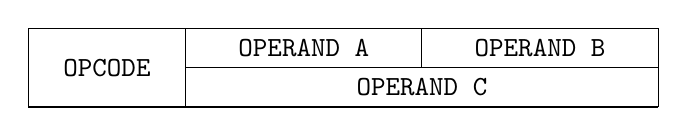
\begin{tikzpicture}
    \draw (0,0) -- (8,0);
    \draw (0,1) -- (8,1);
    \draw (2,0.5) -- (8,0.5);
    \foreach \x in {0,2,8}
        \draw (\x,0) -- (\x,1);
    \draw (5, 0.5) -- (5, 1);
    \node at (1,0.5) {\texttt{OPCODE}};
    \node at (5, 0.25) {\texttt{OPERAND C}};
    \node at (3.5, 0.75) {\texttt{OPERAND A}};
    \node at (6.5, 0.75) {\texttt{OPERAND B}};
\end{tikzpicture}
\caption{Graphic showing the two possible make ups of an instruction.}
\end{figure}

\subsection{Opcodes}

\begin{table}[H]
\centering
\caption{Opcodes and their meanings.}
\begin{tabular}{lll}
Code & Abbreviation & Description \\
\hline
\textbf{Maths} \\
\texttt{0x0} & \texttt{ADD} & Add Operand A or B \\
\texttt{0x1} & \texttt{SUB} & Subtract Operand A from B \\
\textbf{Logical Operations} \\
\texttt{0x2} & \texttt{AND} & Bitwise AND of A and B \\
\texttt{0x3} & \texttt{OR}  & Bitwise OR of A and B \\
\texttt{0x4} & \texttt{NOT} & Bitwise NOT of A \\
\textbf{Control} \\
\texttt{0x5} & \texttt{JMP} & Jump to C \\
\textbf{Movement} \\
\texttt{0x6} & \texttt{STO} & Store the value in the accumulator in C \\
\end{tabular}
\end{table}

\section{Memory}

The memory design is simple, generic, 16-bit memory. It takes three control signals, and if it's given an unexpected signal it returns 1, causing the emulation to stop.

It is connected directly to the Control Unit via an \texttt{address} bus and to the rest of the processor by the \texttt{data} bus.

The size of allocated memory is determined by a \texttt{\#define} called \texttt{MEMORY\_SIZE}.

\begin{table}[H]
\centering
\caption{Control signal names and descriptions for the ALU.}
\begin{tabular}{ll}
	Signal & Description \\
	\hline
	\texttt{MEM\_HIZ} & Don't drive the \texttt{data} bus.\\
	\texttt{MEM\_SET} & Set the memory at the \texttt{address} to the value of the \texttt{data} bus \\
	\texttt{MEM\_ENB} & Drive the \texttt{data} bus with the data stored at the \texttt{address}.\\
\end{tabular}
\end{table}

\subsection{Implementation}

The memory is implemented in the \texttt{memory.c} and \texttt{memory.h} files. The function \texttt{updateMemory()} is called on each clock tick. It consists of a single \texttt{switch case} statement that handles the behavior defined above.

\subsection{Testing}

The memory is tested by setting a reading each possible value to each cell in memory and then reading it back. This test can be found in \verb|test/memory_test.c|.

If the operation fails then some debugging data is output to \texttt{stdout}: the address, data and state of \texttt{memory\_control}.

\section{Arithmetic and Logic Unit}

The ALU takes two inputs, and outputs them onto the data bus when a control input other then \texttt{ALU\_HIZ} is given.

In order to simplify the control unit the ALU takes the same control input as the opcode. This means the only input left to define is \texttt{ALU\_HIZ} which is defined as \texttt{0xFF}.

\subsection{Implementation}

The ALU is implemented in the \texttt{alu.c} and \texttt{alu.h} files. The function \texttt{updateALU()} is called on each clock tick. It consists of a single switch case that switches on the \texttt{alu\_control} input. The data bus is then driven with the output based on the inputs. Input buffering is handled by the control unit.

\subsection{Testing}

ALU testing is handled by \texttt{test/alu\_test.c}. It cycles though each of the operations with all possible inputs and asserts that they are correct. If the inputs are not correct then debugging data is printed to \texttt{stdout}: the type of operation, the two inputs and the output of the ALU as it drives the data bus.

\section{Control Unit}

The control unit is a state machine. 

\section{Wrapper}

\section{Assembler}

\end{document}